\documentclass[a4paper,11pt,danish]{article}

\usepackage[latin1]{inputenc}
\usepackage[T1]{fontenc}
\usepackage[danish]{babel}
\usepackage{url}
\usepackage{lastpage}
\usepackage{bookmark}
\usepackage{fancyhdr}
\usepackage{charter}
\usepackage{rotating}
\usepackage{pdflscape}
\usepackage{appendix}
\pagestyle{fancy}


\date{27. marts 2009}

\newcommand{\mytitle}{Eksamensopgave}
\newcommand{\mysubject}{Menneske-datamaskine interaktion (HCI)}

\newcommand{\HCI}{menneske-datamaskine interaktion}

\newcommand{\mycpr}{180387-1619}

\newcommand{\email}[1]{\href{mailto:#1}{\texttt{#1}}}

\renewcommand{\sectionmark}[1]{\markright{\thesection.\ #1}}

\renewcommand{\appendixtocname}{Bilag}
\renewcommand{\appendixpagename}{Bilag}
\renewcommand{\appendixname}{Bilag}


\title{\huge \mysubject \\ \normalsize \mytitle}

\author{
\begin{tabular}{lr}
  Navn & Julian M�ller \\
  CPR-nummer & 180387-1619 \\
  di-nummer & di080047 \\
  E-mail & \email{di080047@diku.dk} \\
\end{tabular}
}

\fancyhead{}

 	\lhead{}
 	\chead{}
 	\rhead{}
 	\lfoot{}
 	\cfoot{}
 	\rfoot{}

\fancyhead[L]{HCI: \mytitle}
\fancyhead[C]{Julian M�ller}
\fancyhead[R]{\mycpr}
\fancyfoot[L]{\rightmark}
\fancyfoot[R]{Side \thepage \ af \pageref{LastPage}}

\begin{document}

\maketitle
\tableofcontents

\pagebreak


\section{Kursusaktivitet dokumenteret ved syv ugeopgaver}
\label{sec:kurs-dokum-ved}

De syv ugeopgaver kan findes i de vedlagte bilag (s. \pageref{appendic}).

Overordnet set er jeg ret tilfreds med mine ugeopgaver. Jeg synes jeg
er kommet godt rundt omkring de stillede krav i alle opgaverne, og har
f�et udf�rt nogle gode analyser og forbedringsforslag.

Aspekterne, jeg generelt ikke har v�ret helt tilfreds med i mine
opgaver har v�ret de forskellige brugerunders�gelser. Jeg synes det
var sv�rt at retf�rddigg�re s� ``store'' unders�gelser for s� sm�
opgaver. Jeg synes ikke at den store m�ngde tid det ville tage fx at
lave en komplet kontekstuel unders�gelse var retf�rdiggjort - hverken
for mig selv eller for testpersonerne. Fra et teoretisk synsspunkt
kunne jeg godt have brugt mere tid p� unders�gelserne, for at f� et
mere repr�sentativt resultat.

Den unders�gelse jeg var mest tilfreds med, er at finde i min
ugeopgave 4, som ogs� er den opgave jeg er mest tilfreds med. Opgaven
var sp�ndende og ved hj�lp af unders�gelsen og de to stillede konkrete
scenarier fandt jeg nogle gode krav til det �nskede rejsesystem inden
for \emph{PACT}. Den kontekstuelle unders�gelse lagde ogs� et godt
grundlag for det konkrete scenarie der skulle skrives. Endvidere blev
mit endelige redesigforslag vellykket og passede godt til den stillede
opgave samt de forskellige brugsscenarier der var.

Det svageste punkt ved min opgave var den gennemg�ende mangel p�
referencer jeg har f�et lavet i mine ugeopgaver. I retrospekt ville
flere referencer til l�reb�ger, artikler eller lignende have gavnet opgaven,
da det dermed ville have v�ret tydelgiere at mine id�er ikke blot var
grebet ud af den bl� luft, men byggede p� videnskabelig forskning
inden for \HCI.
\include{del-b.tex}
%%% Local Variables: 
%%% mode: latex
%%% TeX-master: "julian_moeller_eksamen"
%%% End: 

\appendix
\appendixpage
\addappheadtotoc

\label{appendix}

\section{Figurer}
\label{sec:figurer}

\begin{figure}[h]
  \centering
  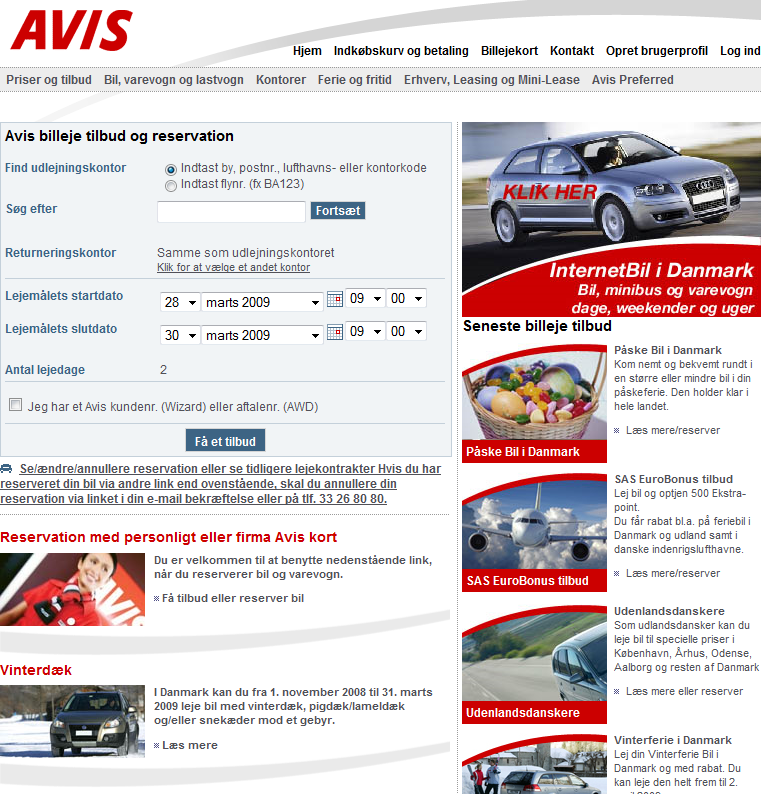
\includegraphics[width=13cm]{figures/avis_dk.png}
  \caption{AVIS' nuv�rende webside (marts 2009)}
  \label{fig:avisbilovs}
\end{figure}

\begin{figure}[h]
  \centering
  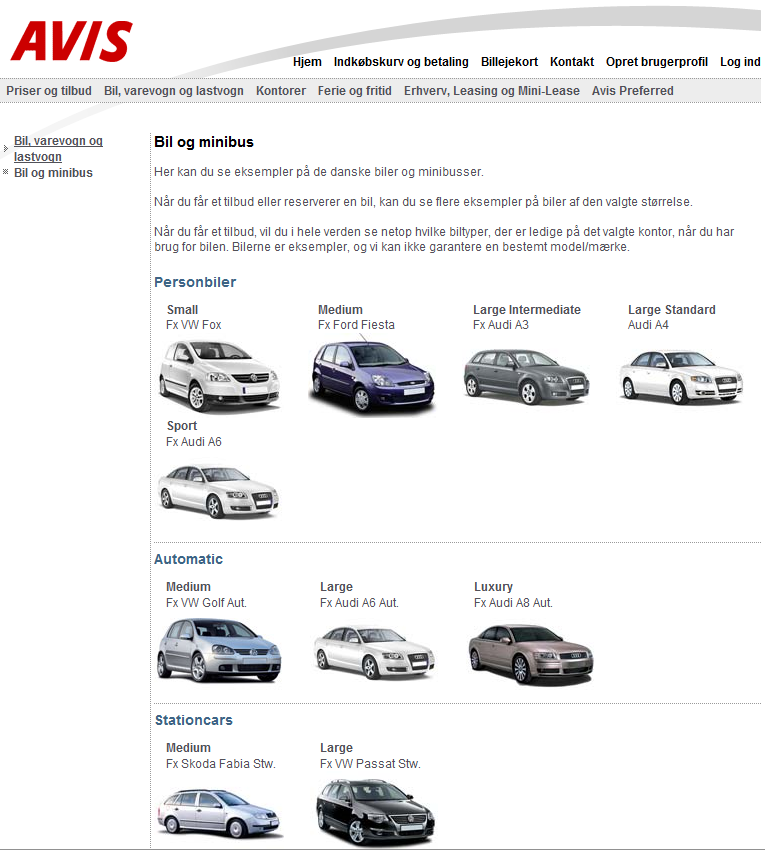
\includegraphics[width=13cm]{figures/avis_biloversigt.png}
  \caption{Biloversigten p� AVIS' nuv�rende webside (marts 2009)}
  \label{fig:avisdk}
\end{figure}

\begin{figure}[h]
  \centering
  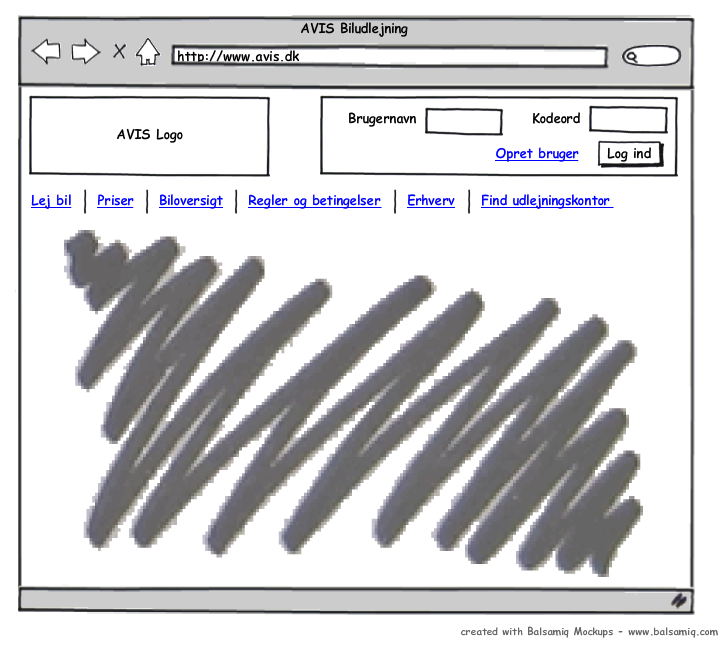
\includegraphics[width=13cm]{figures/menubar_mockup.png}
  \caption{Forslag til �ndring af menulinjen p� AVIS' webside}
  \label{fig:menubar}
\end{figure}

\begin{figure}[h]
  \centering
  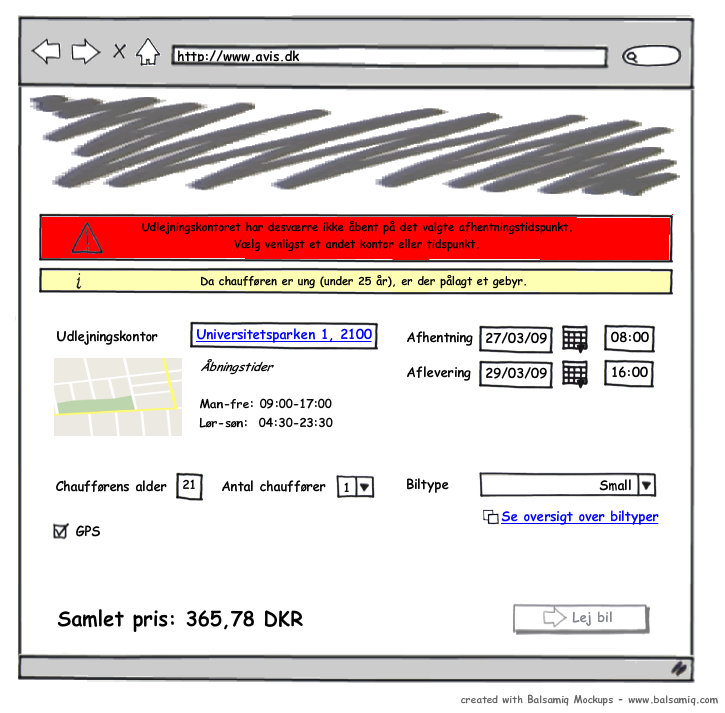
\includegraphics[width=13cm]{figures/search_mockup.png}
  \caption{Forslag til �ndring af s�geinterfacet p� AVIS' webside}
  \label{fig:search}
\end{figure}

\begin{figure}[h]
  \centering
  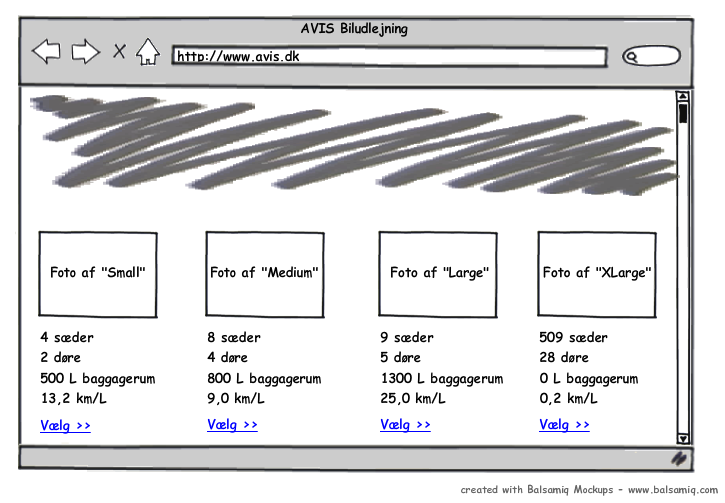
\includegraphics[width=13cm]{figures/choosecar_mockup.png}
  \caption{Forslag til �ndring af biloversigten p� AVIS' webside}
  \label{fig:choosecar}
\end{figure}

\clearpage


\section{Ugeopgaver}
\label{sec:ugeopgaver}


\end{document}